\documentclass[a4paper,14pt]{extarticle}

\usepackage[utf8x]{inputenc}
\usepackage[T1,T2A]{fontenc}
\usepackage[russian]{babel}
\usepackage{hyperref}
\usepackage{indentfirst}
\usepackage{here}
\usepackage{array}
\usepackage{graphicx}
\usepackage{caption}
\usepackage{subcaption}
\usepackage{chngcntr}
\usepackage{amsmath}
\usepackage{amssymb}
\usepackage{pgfplots}
\usepackage{pgfplotstable}
\usepackage[left=2cm,right=2cm,top=2cm,bottom=2cm,bindingoffset=0cm]{geometry}
\usepackage{multicol}
\usepackage{askmaps}
\usepackage{titlesec}
\usepackage{listings}
\usepackage{color}
\usepackage{courier}

\definecolor{green}{rgb}{0,0.6,0}
\definecolor{gray}{rgb}{0.5,0.5,0.5}
\definecolor{purple}{rgb}{0.58,0,0.82}

\lstset{
	language=Verilog,
	backgroundcolor=\color{white},   
	basicstyle=\small\ttfamily,
	commentstyle=\color{green},
	keywordstyle=\color{blue},	
	numberstyle=\tiny\color{gray},
	stringstyle=\color{purple},
	breakatwhitespace=false,
	breaklines=true,
	captionpos=b,
	keepspaces=true,
	numbers=left,
	numbersep=5pt,
	showspaces=false,
	showstringspaces=false,
	showtabs=false,
	tabsize=4,
	frame=single,
	inputpath={../quartus/},
	literate={~} {$\sim$}{1}
}

\renewcommand{\le}{\ensuremath{\leqslant}}
\renewcommand{\leq}{\ensuremath{\leqslant}}
\renewcommand{\ge}{\ensuremath{\geqslant}}
\renewcommand{\geq}{\ensuremath{\geqslant}}
\renewcommand{\epsilon}{\ensuremath{\varepsilon}}
\renewcommand{\phi}{\ensuremath{\varphi}}
\renewcommand{\thefigure}{\arabic{figure}} 	
\renewcommand*\not[1]{\overline{#1}}

\titleformat*{\section}{\large\bfseries} 
\titleformat*{\subsection}{\normalsize\bfseries} 
\titleformat*{\subsubsection}{\normalsize\bfseries} 
\titleformat*{\paragraph}{\normalsize\bfseries} 
\titleformat*{\subparagraph}{\normalsize\bfseries} 

\counterwithin{figure}{section}
\counterwithin{equation}{section}
\counterwithin{table}{section}
\newcommand{\sign}[1][5cm]{\makebox[#1]{\hrulefill}}
\graphicspath{{../pics/}}
\captionsetup{justification=centering,margin=1cm}
\def\arraystretch{1.3}
\setlength\parindent{5ex}
\titlelabel{\thetitle.\quad}

\begin{document}

\begin{titlepage}
\begin{center}
	Санкт-Петербургский Политехнический Университет Петра Великого\\[0.3cm]
	Институт компьютерных наук и технологий \\[0.3cm]
	Кафедра компьютерных систем и программных технологий\\[4cm]
	
	\textbf{ОТЧЕТ}\\ 
	\textbf{по лабораторной работе}\\[0.5cm]
	\textbf{SystemVerilog №4}\\[0.1cm]
	Автоматизация проектирования\\ дискретных устройств\\[4.0cm]
\end{center}

\begin{flushright}
	\begin{minipage}{0.45\textwidth}
		\textbf{Работу выполнил студент}\\[3mm]
		группа 33501/4 \hspace*{9mm} Дьячков В.В.\\[5mm]
		\textbf{Преподаватель}\\[5mm]
		\sign[1.5cm] \hspace*{1mm} к.т.н., доц. Филиппов А.С. \\[5mm]
	\end{minipage}
\end{flushright}

\vfill

\begin{center}
	Санкт-Петербург\\
	\the\year
\end{center}
\end{titlepage}

\addtocounter{page}{1}
\counterwithin{lstlisting}{section}

\tableofcontents
\listoffigures
\newpage

\section{Цель работы}

\begin{itemize}
	\item Закрепление знаний, полученных в SignalTapII 1, продолжение изучения возможностей встроенного логического анализатора SignalTapII пакета QuartusII;
	\item Получение навыков анализа реальных процессов с помощью логического анализатора SignalTapII пакета QuartusII;
	\item Исследование дребезга контактов движкового переключателя с помощью логического анализатора;
	\item Реализация и исследование работы схемы борьбы с дребезгом контактов.
\end{itemize}

\section{Подготовка проекта для исследования дребезга контактов движкового переключателя}

\subsection{Создание и ввод проекта}

На рис. \ref{fig:source} изображена схема для исследования дребезга контактов механического движкового переключателя, дополненная логическим анализатором, фиксирующим требуемые сигналы в схеме. Движковый переключатель \code{sw} подключен к синхровходу восьмиразрядного счетчика \code{cnt}. Счетчик подсчитывает число переходов \code{0=>1} при переключении движкового переключателя из \code{0} в \code{1} и обратно. Число переходов (импульсов дребезга) отображается на светодиодах \code{led[7..0]}. Сигнал от кнопки \code{pb} осуществляет сброс счетчика.

\begin{figure}[H]
	\begin{center}
		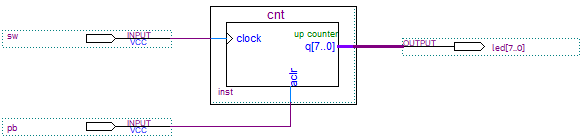
\includegraphics[scale=0.95]{source}
		\caption{Исследуемый проект}
		\label{fig:source}
	\end{center}
\end{figure}
\vspace{-1cm}

\subsection{Создание экземпляра логического анализатора ELA1}

На рис. \ref{fig:stp_1} изображено окно SignalTapII Logic Analyzer со списком целей в созданном \code{stp}-файле.
\vspace{-0.5cm}
\begin{figure}[H]
	\begin{center}
		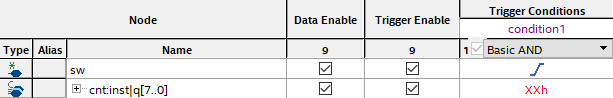
\includegraphics[width=0.9\textwidth]{stp}
		\caption{Список целей в SignalTapII Logic Analyzer}
		\label{fig:stp_1}
	\end{center}
\end{figure}

\subsection{Конфигурирование СБИС}

\section{Исследование дребезга контактов движкового переключателя}

\subsection{Исследование дребезга при переключениях из 0 => 1}

\subsection{Исследование дребезга при переключениях из 1 => 0}

\section{Реализация устройства защиты от дребезга}

\section{Выводы}

\end{document}